
\documentclass[12pt]{article}
\usepackage[a4paper, margin=.30in]{geometry}
\usepackage{graphicx ,
            wrapfig,
            xcolor, 
            enumerate,
            amsmath,
			fontenc,
			tcolorbox,circuitikz
            }

\newcommand\headerMe[2]{\noindent{}#1\hfill#2}
\renewcommand{\thesection}{\Roman{section}}

\author{Zakaria HAOUZAN}
\date{\today}

\begin{document}
% headers --------------
\headerMe{Matière : Physique-Chimie}{Professeur : Zakaria HAOUZAN}\\
\headerMe{Unité : Electricité }{Établissement : Lycée SKHOR qualifiant}\\
\headerMe{Niveau : 2BAC-SM-PC}{Heure : 6H}\\

% ------Content ________
\begin{center}

    \Large{Leçon $N^{\circ} 6 $: \color{red} Dipôle RC }
\end{center}

%\begin{wrapfigure}[10]{r}{0.5\textwidth}
%    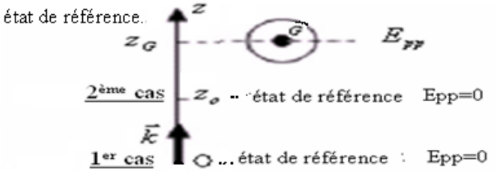
\includegraphics[width=0.5\textwidth]{./img/img00.png}
%\end{wrapfigure}

\section{Le condensateur : }
\subsection{Définition : }
\begin{wrapfigure}{r}{0000.000001\textwidth}
 
\begin{circuitikz}
  \draw (0,0) 
        to node[below,pos=2]{$+q$} node[above,pos=2]{$+$} (0.5,0) 
        to [C, l^=$C$] (2.5,0) 
        to node[below,pos=-1]{$-q$} node[above,pos=-1]{$-$} (3,0) ;
\end{circuitikz}
\end{wrapfigure}


Un condensateur est constitué de deux conducteurs en regard appelés armatures séparés par un isolant qu'on appelle diélectrique
(comme l'air, le verre, le plystyrène, le plastique ou le papier paraffiné...etc.qui sont des substances isolantes).

Les armatures du condensateur peuvent prendre divers formes géométrique.


\subsection{Charge et décharge d'un condensateur : }

\begin{wrapfigure}[10]{r}{0.5\textwidth}
	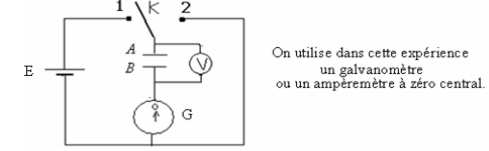
\includegraphics[width=0.5\textwidth]{./img/charge_00.png}
	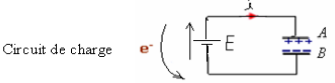
\includegraphics[width=0.5\textwidth]{./img/charge_001.png}
\end{wrapfigure}


\subsubsection{Charge d'un condensateur: Expérience }
On utilise un générateur source de tension continue de force éléctromotrice E et on réalisé le montage suivant: 




\begin{itemize}
	\item On bascule l'interrupteur K à la position (1).

	\item On observe que l'ampèremètre indique le passage d'un courant électrique durant un temps très court et que le voltmètre indique
que la tension aux bornes du condensateur UAB=E.

\item On dit que le condensateur est chargé et le courant électrique qui passe dans le circuit s'appelle courant de charge.

\end{itemize}

\section*{Interprétation: }
\begin{itemize}
	\item Le courant de charge résulte d'un déplacement des électrons de l'armature A vers l'armature B du condensateur, et à cause de l'existence du diélectrique entre les armatures, les électrons s'accumulent sur l'armature B.

	\item L'armature A perd le même nombre d'électrons gagnés par l'armature B et condensateur devient chargé. $q=q_A=-q_B$

	\item Une fois chargé, le condensateur conserve la charge électrique "q" sur ses armatures et la tension uAB=E entre
ses bornes, même lorsqu'on le débranche.

\end{itemize}


\subsubsection{Décharge d'un condensateur: Expérience }
Lorsque le condensateur est chargé on bascule l'interrupteur K à la position (2). On constate la déviation de l'aiguille du
galvanomètre dans le sens contraire pendant un temps très court et le voltmètre indique une annulation rapide de la tension aux
bornes du condensateur.

\section*{Interprétation: }

\begin{wrapfigure}{r}{0.5\textwidth}
	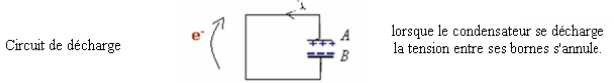
\includegraphics[width=0.5\textwidth]{./img/decharge_00.png}
\end{wrapfigure}

En déplaçant l'interrupteur à la position (2) on relie les armatures entre elles .Les électrons accumulés sur l'armature B reviennent à
l'armature A et un courant de décharge apparait dans le circuit dans le sens inverse du courant de charge.

\subsubsection{Relation entre la charge et l'intensité du courant : }

L'intensité du courant électrique est le débit de porteurs de charges qui traverse la section du conducteur par unité de temps.

\begin{itemize}
	\item Dans un courant continue On a : $I=\frac{q}{t}$
	\item Dans un courant variable On a : $i=\frac{dq}{dt}$
	\item Dans le cas du condensateur  On a : $i=\frac{dq}{dt} = \frac{q}{t}$
\end{itemize}


\subsubsection{Relation entre la charge et la tension d'un condensateur : (charge du condensateur avec un courant constant) }

\begin{wrapfigure}{r}{0.2\textwidth}
	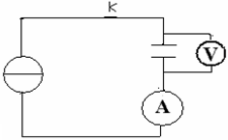
\includegraphics[width=0.2\textwidth]{./img/circuit00.png}
\end{wrapfigure}


On réalise le montage de la figure suivante en utilisant un générateur de courant (qui débite un courant électrique constant quelle
que soit la tension entre ses bornes) .Puis on ferme l'interrupteur et en même temps on déclenche le chronomètre.

L'ampèremètre indique l'intensité du courant dans le circuit $I_0=0,3\mu.A$. 

On mesure la tension entre les bornes du condensateur

après chaque cinq secondes et en utilisant la relation : $q=I_0.t$ , on détermine la charge q du condensateur à chaque instant.

Tableau des valeurs: 
\begin{center}
   \begin{tabular}{ |c|c|c|c|c|c|c|c|c|c|c| }
	  \hline
	  $t$       &0   & 5    & 10 & 15   & 20  &25  & 30  & 35 & 40 & 45 \\
	  \hline
	  $U_c(V)$  & 0  &0,25  & 0,5& 0,75&1     &1,25 &1,5 &1,75&2	&2,25  \\\hline
	  $q(\mu.C)$& 0  &  1,5 & 3  &   4,5& 6   &7,5& 9   &10,5&12  &13,5\\
\hline
\end{tabular}
\end{center}
Représentation de la courbe d'évolution de la charge q en fonction du temps:

\begin{center}
	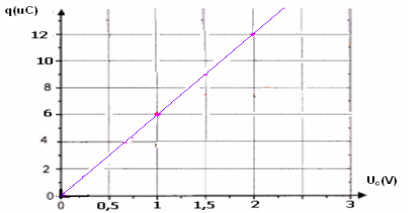
\includegraphics[width=0.5\textwidth]{./img/q(t).png}
\end{center}

\begin{itemize}
	\item La charge q du condensateur est proportionnelle à la tension entre ses bornes, le coefficient de proportionnalité est une constante
qui caractérise le condensateur notée C, est appelée : capacité du condensateur, elle s’exprime en farad (F).
$$q = C.U_c$$

\item Graphiquement la capacité du condensateur utilisé dans cette expérience est égale au coefficient directeur $C = \frac{\Delta{q}}{\Delta{U}} = 6\mu.F$

\end{itemize}


\section{Association des condensateurs : }

\subsection{Association en parallèle : }
Soient deux condensateurs de capacités C1 et C2 montés en parallèle et soit C la capacité du condensateur équivalent (qui peut les
remplacer et jouer leur rôle)

\begin{center}
	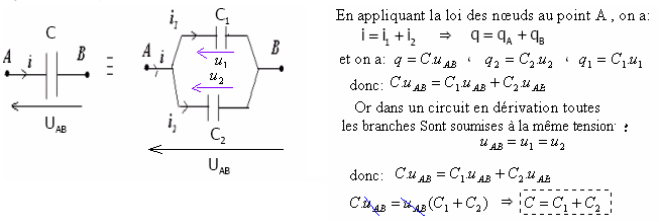
\includegraphics[width=0.75\textwidth]{./img/parallele.png}
\end{center}





La capacité C du condensateur équivalent à un ensemble de condensateurs de capacités C1, C2,C3.......Cn montés en parallèle $C=\sum C_i$

Remarque : le montage en parallèle sert à faire augmenter la capacité du condensateur.

\subsection{Association en série : }
Soient deux condensateurs de capacités C1 et C2 montés en série et soit C la capacité du condensateur équivalent (qui peut les remplacer et jouer leur rôle)


\begin{center}
	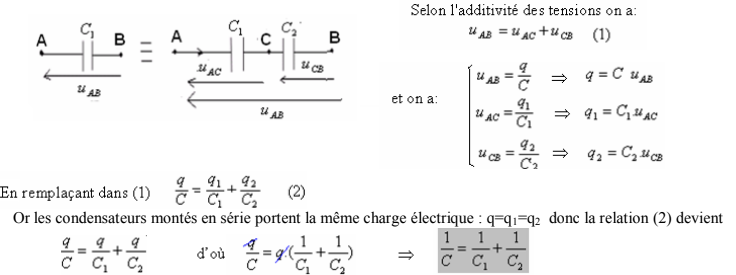
\includegraphics[width=0.8\textwidth]{./img/serie.png}
\end{center}


La capacité C du condensateur équivalent à un ensemble de condensateurs de capacités C1, C2,C3.......Cn montés en série : $\frac{1}{C} = \sum \frac{1}{C_i}$

\section{Réponse d'un dipôle  RC à un échelon de tension: }

\subsection{Réponse d'un dipôle  RC à un échelon montant de tension: (Charge d'un condensateur) }
\section*{l'équation différentielle:  }
On dit qu'un dipôle est soumis à un échelon montant de tension, si la tension entre ses bornes varie instantanément d'une valeur
nulle à une valeur constante E.


\begin{center}
	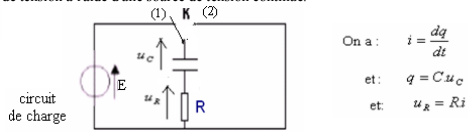
\includegraphics[width=0.4\textwidth]{./img/chargeRC.png}
	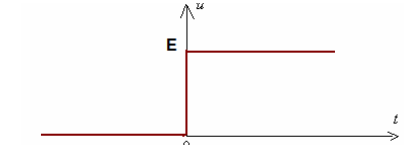
\includegraphics[width=0.3\textwidth]{./img/montant.png}
\end{center}



\begin{itemize}
	\item On monte en série un conducteur ohmique de résistance R et un condensateur de capacité C et on obtient un dipôle RC puis on le
soumis à un échelon de montant de tension à l'aide d'une source de tension continue.


\item On représente les différentes tensions en respectant la convention récepteur et la convention générateur.


	\item en convention récepteur la tension u et le courant i sont de sens contraire.
	\item En convention générateur la tension u et le courant i sont de même sens.
\end{itemize}
\underline{En appliquant la loi d'additivité des tensions on a: }

$U_R + U_C = E$ donc $$RC.\frac{du_c}{dt} + u_c = E$$
On pose $\tau = R.C$  constante de temps du dipôle RC.

$$\tau.\frac{du_c}{dt} + u_c = E$$

C'est l'équation différentielle que vérifie la tension aux bornes du condensateur durant la charge. 


\section*{Solution de l'équation différentielle:}
La solution générale de cette équation différentielle est de la forme : $u_c = A.e^{-\alpha.t} + B$

\begin{itemize}
	\item Les constantes : A ,B et $\alpha$ se déterminent en remplaçant et utilisant les conditions initiales.
	\item sa derivée: $\frac{du_c}{dt} = -\alpha.A.e^{-alpha.t}$ (1)
	\item En remplaçant la solution uc et sa dérivée, l’équation différentielle : $A = -E$ et B = E.
	\item Donc la solution de l'équation différentielle : 
\end{itemize}

$$u(t) = E(1-e^{-\frac{t}{\tau}})$$ avec $\tau = R.C$


\begin{center}

	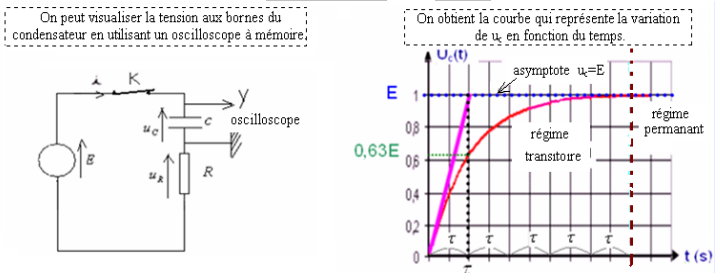
\includegraphics[width=0.8\textwidth]{./img/solution_charge.png}
\end{center}

\begin{itemize}
	\item On constate l'existence de deux régimes:
	\item Un régime transitoire durant lequel la tension aux bornes du condensateur varie de 0 à E.
\item Un régime permanent au cours duquel la tension aux bornes du condensateur devient constante : uc=E.


\end{itemize}

\section*{Unité de la constante de temps:}
Montros que le produit RC est homogène à un temps. 
L’analyse dimensionnelle conduit à : $$[\tau] = [R].[C]$$
$$[\tau] = [t]$$


\section*{Détermination graphique de la valeur de: $\tau$}

1 ère méthode: En remplaçant $t=\tau$ dans l'expression de la tension on obtient $u_c = E(1-e^{-1}) = 0,63E$

2  ème méthode:
 La tangente à la courbe à t=0 se coupe avec l'asymptote uc=E à l'instant

 \section*{Expression de l'intensité du courant dans le circuit: }

\begin{wrapfigure}{r}{0.2\textwidth}
	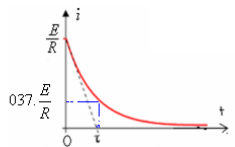
\includegraphics[width=0.2\textwidth]{./img/current_courbe01.png}
\end{wrapfigure}


 On a d'après la loi d'additivité des tensions: $u_r + U_c =E$ donc $$i= \frac{E}{R}.e^{\frac{-t}{\tau}}$$

 car $u(t) = E(1-e^{\frac{-t}{\tau}})$

 autre méthode: $i = \frac{dq}{dt} $ donc $$i= \frac{E}{R}.e^{\frac{-t}{\tau}}$$



\subsection{Réponse d'un dipôle  RC à un échelon descendant de tension: (décharge d'un condensateur) }

\subsubsection{l'équation différentielle:  }
On dit qu'un dipole est soumis à un échelon descendant de tension, si la tension entre ses bornes varie instantanément d'une
valeur constante E à une valeur nulle .

Lorsque le condensateur est chargé on bascule l'interrupteur K à la position (2)

On représente les différentes tensions en respectant la convention récepteur et la convention générateur.


\begin{center}

	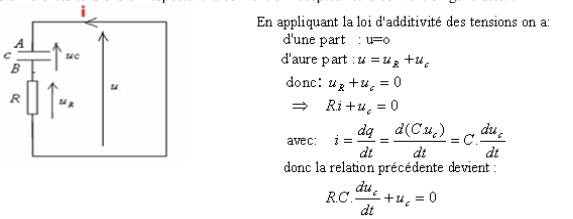
\includegraphics[width=0.7\textwidth]{./img/decharge_RC01.png}
\end{center}

On pose $\tau = R.C$ donc $\tau.\frac{du_c}{dt} + u_c = 0$

C'est l'équation différentielle que vérifie la tension aux bornes du condensateur durant la décharge.

\subsubsection{Solution de l'équation différentielle: }

La solution générale de cette équation différentielle est de la forme $u_c(t) = A.e^{-\alpha .t} + B $

La solution générale de cette équation différentielle est : $$u_c(t) = E.e^{-\frac{r}{\tau}}$$

\subsubsection{Détermination graphique de la valeur de $\tau$}


1 ère méthode: En remplaçant $t = \tau$ dans l'expression de la tension on obtient : $u_c(\tau) =  0,37E$

2 ème méthode: La tangente à la courbe à $t=0$ se coupe avec l'asymptote uc=E à l'instant $t=\tau$

\subsubsection{Expression de l'intensité du courant dans le circuit: }

On a d'après la loi d'additivité des tensions: $u_r + U_c = 0$ donc $i = -\frac{E}{R}.e^{-\frac{-t}{\tau}}$.

\section{Energie électrique emagasiné dans un condensateur : }


On bascule l'interrupteur K à la position (1) et on le laisse un temps suffisant pour que le condensateur soit chargé puis on le
bascule à la position (2).

On constate que le moteur fonctionne et le corps suspendu au fil monte d'une hauteur h.

La montée du corps et sa réception d’une énergie de potentielle s'explique par l'existence de l'énergie électrique qui a été reçue par
le condensateur pendant la charge.

Donc le condensateur peut emmagasiner l'énergie électrique pour la restituer au moment du besoin.


\subsection{Expression de l'énergie emmagasinée dans un condensateur : }

Soit Ee l'énergie électrique emmagasinée dans un condensateur: 

%wfg---------------------------------------------------------------sf 
%\begin{center}
   %\begin{tabular}{ |c|c|c|c|c|c|c| }
      %\hline
      %km & hm & dam & \bf{m} & dm & cm & mm \\
      %\hline
        %&   &    &  &   &   & \\
%\hline
%\end{tabular}
%On place un seul nombre dans chaque case.
%\end{center}
%\begin{center}
   %\begin{tabular}{ |c|c|c|c|c|c|c| }
      %\hline
      %$km^2$ & $hm^2$ & $dam^2$ & \bf{$m^2$} & $dm^2$ & $cm^2$ & $mm^2$ \\
      %\hline
        %&   &    &  &   &   & \\
%\hline
%\end{tabular}
%\end{center}


\end{document}

